% Build from this directory with: tectonic main.tex
% The Chinese paper body lives in paper-body.tex.
% The bibliography is reused directly from ../paper/references.bib.
\documentclass[UTF8,a4paper,zihao=5,fontset=none]{ctexart}

\usepackage[top=1.85cm,bottom=2.0cm,left=2.2cm,right=2.2cm,headheight=15pt,headsep=0.55cm]{geometry}
\usepackage{fontspec}
\usepackage{amsmath}
\usepackage{unicode-math}
\usepackage{booktabs}
\usepackage{longtable}
\usepackage{tabularx}
\usepackage{array}
\usepackage{graphicx}
\usepackage{float}
\usepackage{xurl}
\usepackage{xcolor}
\usepackage{hyperref}
\usepackage{fancyhdr}
\usepackage{fancyvrb}
\usepackage{enumitem}
\usepackage{caption}
\usepackage{xspace}
\usepackage{microtype}
\usepackage{tikz}
\usetikzlibrary{arrows.meta,positioning,calc}

\setCJKmainfont[Script=Default,AutoFakeBold=2,AutoFakeSlant=.2]{Songti SC}
\setCJKsansfont[Script=Default,AutoFakeBold=2]{PingFang SC}
\setCJKmonofont{PingFang SC}
\setmainfont{Times New Roman}
\setsansfont{Arial}
\setmonofont{Menlo}
\setmathfont{STIX Two Math}

\definecolor{hyperblue}{HTML}{0000EE}
\definecolor{inkblue}{HTML}{202020}
\definecolor{paperblue}{HTML}{F2F2F2}
\definecolor{lineblue}{HTML}{777777}
\definecolor{accentorange}{HTML}{555555}
\definecolor{softorange}{HTML}{F5F5F5}
\definecolor{resultgreen}{HTML}{333333}
\definecolor{softgreen}{HTML}{EEEEEE}
\definecolor{mutedred}{HTML}{666666}
\definecolor{softred}{HTML}{F7F7F7}
\definecolor{textgray}{HTML}{333333}

\hypersetup{
  unicode=true,
  hypertexnames=false,
  colorlinks=true,
  linkcolor=hyperblue,
  citecolor=hyperblue,
  urlcolor=hyperblue,
  pdftitle={当更好的检索带来更差的答案：跨十八个研究方向的下游门控生命周期记忆},
  pdfauthor={},
  pdfsubject={面向多轮长任务的生命周期记忆自优化研究},
  pdfkeywords={生命周期记忆, 记忆自优化, 纠错链, 下游门控, MemoryCore}
}
\urlstyle{same}

\setlength{\parindent}{2em}
\setlength{\parskip}{0.10em}
\linespread{1.11}
\setlength{\LTpre}{0.45em}
\setlength{\LTpost}{0.45em}
\renewcommand{\arraystretch}{1.08}
\setlist{nosep,leftmargin=2.4em}
\setcounter{secnumdepth}{3}
\setcounter{tocdepth}{2}
\emergencystretch=2em
\allowdisplaybreaks

\ctexset{
  section = {
    format = \centering\Large\bfseries\color{black},
    beforeskip = 1.65ex plus .4ex,
    afterskip = 1.0ex
  },
  subsection = {
    format = \large\bfseries\color{black},
    beforeskip = 1.2ex plus .25ex,
    afterskip = 0.55ex
  },
  subsubsection = {
    format = \normalsize\bfseries\color{black},
    beforeskip = 0.9ex plus .2ex,
    afterskip = 0.32ex
  }
}

\captionsetup{
  font=small,
  labelfont={color=black},
  textfont={color=black},
  skip=5pt
}

\pagestyle{fancy}
\fancyhf{}
\fancyhead[L]{\small 调研报告}
\fancyhead[R]{\small 下游门控生命周期记忆}
\fancyfoot[C]{\thepage}
\renewcommand{\headrulewidth}{0.4pt}
\renewcommand{\footrulewidth}{0pt}
\fancypagestyle{plain}{
  \fancyhf{}
  \fancyhead[L]{\small 调研报告}
  \fancyhead[R]{\small 下游门控生命周期记忆}
  \fancyfoot[C]{\thepage}
  \renewcommand{\headrulewidth}{0.4pt}
  \renewcommand{\footrulewidth}{0pt}
}

\newcommand{\base}{\textsf{Base}\xspace}
\newcommand{\vone}{\textsf{V1}\xspace}
\newcommand{\vtwo}{\textsf{V2}\xspace}

\newenvironment{paperabstract}
  {\begin{center}\vspace{1.25cm}{\large\bfseries 摘要}\end{center}\vspace{0.45em}\small\noindent}
  {\par\vspace{0.75em}\noindent\textbf{关键词：}生命周期记忆；记忆自优化；纠错链；下游门控；多轮编程 Agent\par}

\newcommand{\frameworkfigure}{\begin{figure}[htbp]
\centering
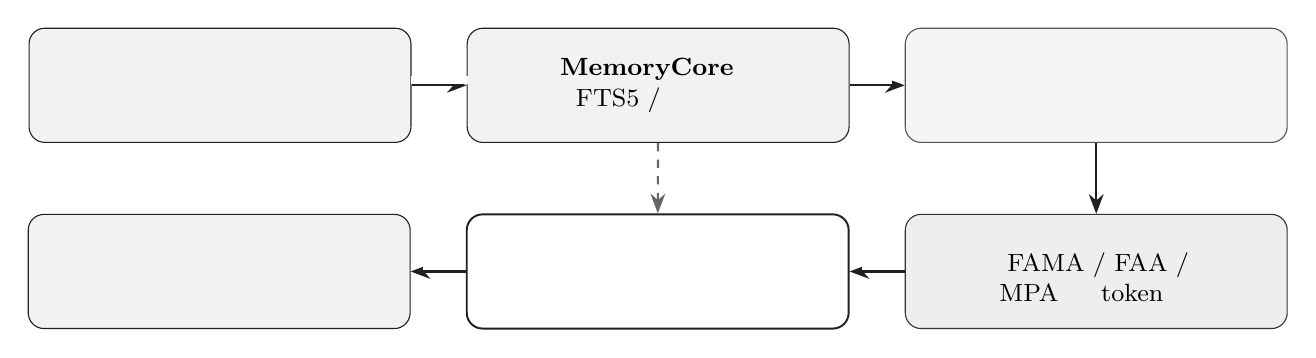
\begin{tikzpicture}[
  font=\small,
  box/.style={
    draw=inkblue,
    fill=paperblue,
    rounded corners=2mm,
    minimum height=1.45cm,
    text width=4.25cm,
    align=center,
    inner sep=3mm
  },
  accent/.style={box,draw=accentorange,fill=softorange},
  gate/.style={box,draw=resultgreen,fill=softgreen},
  decision/.style={box,draw=inkblue,fill=white,line width=0.7pt},
  flow/.style={-{Stealth[length=2.5mm]},draw=inkblue,line width=0.8pt},
  fallback/.style={-{Stealth[length=2.5mm]},draw=mutedred,dashed,line width=0.8pt},
  note/.style={font=\scriptsize,fill=white,inner sep=1.5pt,text=textgray}
]
  \node[box] (session) {\textbf{多轮会话与反馈}\\纠错、重述、状态变化、任务结果};
  \node[box,right=7mm of session] (base) {\textbf{MemoryCore 基座}\\FTS5 / 向量召回与固定候选池};
  \node[accent,right=7mm of base] (sidecar) {\textbf{生命周期旁路}\\版本链、失效账本、重定向与回填};

  \node[gate,below=9mm of sidecar] (gates) {\textbf{冻结晋升门槛}\\FAMA / FAA / MPA、置信区间、token 与时延};
  \node[decision,left=7mm of gates] (decision) {\textbf{策略决策}\\通过：晋升候选\quad 失败：保留现行策略};
  \node[box,left=7mm of decision] (answer) {\textbf{受控注入与答案}\\记录所用策略、成本、证据与回退原因};

  \draw[flow] (session) -- node[note,above]{低成本反馈提出候选} (base);
  \draw[flow] (base) -- node[note,above]{排序候选} (sidecar);
  \draw[flow] (sidecar) -- node[note,right]{候选上下文} (gates);
  \draw[flow] (gates) -- node[note,above]{下游判定} (decision);
  \draw[flow] (decision) -- node[note,above]{固定预算} (answer);
  \draw[fallback] (base) -- node[note,right]{关闭、超时、损坏或循环} (decision);
\end{tikzpicture}
\caption{下游门控生命周期记忆框架。反馈只负责提出候选；冻结的答案质量与成本门槛决定是否晋升。旁路异常时，整次调用精确回退至基座结果。}
\label{fig:lifecycle-framework}
\end{figure}
}
\newcommand{\researchmapfigure}{\begin{figure}[htbp]
\centering
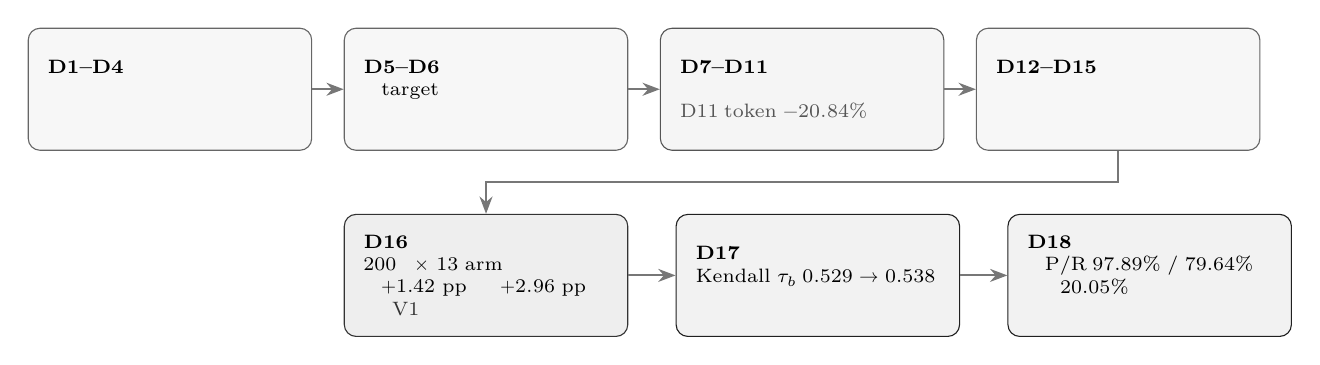
\begin{tikzpicture}[
  font=\scriptsize,
  phase/.style={
    draw=inkblue,
    fill=paperblue,
    rounded corners=1.5mm,
    minimum height=1.55cm,
    text width=3.10cm,
    align=left,
    inner sep=2.5mm
  },
  rejected/.style={phase,draw=mutedred,fill=softred},
  efficiency/.style={phase,draw=accentorange,fill=softorange},
  confirmed/.style={phase,draw=resultgreen,fill=softgreen},
  diagnostic/.style={phase,draw=inkblue,fill=paperblue},
  flow/.style={-{Stealth[length=2.2mm]},draw=lineblue,line width=0.75pt}
]
  \node[rejected] (d14) {\textbf{D1--D4｜失效与预算}\\屏蔽、路由、回填、装箱\\\textcolor{mutedred}{拒绝或近失}};
  \node[rejected,right=4mm of d14] (d56) {\textbf{D5--D6｜状态投影}\\显式 target 与支配守卫\\\textcolor{mutedred}{仅后验证据}};
  \node[efficiency,right=4mm of d56] (d711) {\textbf{D7--D11｜变化与过程}\\状态差分、轨迹、证据压缩\\\textcolor{accentorange}{D11：token $-20.84\%$}};
  \node[rejected,right=4mm of d711] (d1215) {\textbf{D12--D15｜证据修复}\\扩展、残差、前提反驳\\\textcolor{mutedred}{质量或覆盖失败}};

  \node[confirmed,below=8mm of d56] (d16) {\textbf{D16｜广覆盖因果检验}\\200 题 $\times$ 13 arm\\全量 $+1.42$ pp；遗忘子集 $+2.96$ pp\\\textcolor{resultgreen}{条件确认 V1}};
  \node[diagnostic,right=6mm of d16] (d17) {\textbf{D17｜代理诊断}\\Kendall $\tau_b$：0.529 $\rightarrow$ 0.538\\\textcolor{mutedred}{未达到替代门槛}};
  \node[diagnostic,right=6mm of d17] (d18) {\textbf{D18｜纯文本构链}\\事件 P/R：97.89\% / 79.64\%\\链接精确率：20.05\%\\\textcolor{inkblue}{仅事件检测成立}};

  \draw[flow] (d14) -- (d56);
  \draw[flow] (d56) -- (d711);
  \draw[flow] (d711) -- (d1215);
  \draw[flow] (d1215.south) -- ++(0,-4mm) -| (d16.north);
  \draw[flow] (d16) -- (d17);
  \draw[flow] (d17) -- (d18);
\end{tikzpicture}
\caption{D1--D18 的研究筛选路径。早期方向用于缩小机制空间；D16 负责广覆盖确认，D17 诊断代理失配，D18 检验脱离 oracle 元数据后的自动构链边界。}
\label{fig:research-map}
\end{figure}
}

\begin{document}

\thispagestyle{empty}
\begin{center}
  \vspace*{1.35cm}
  {\bfseries\zihao{2} 当更好的检索带来更差的答案\par}
  \vspace{0.55em}
  {\zihao{-3} 跨十八个研究方向的下游门控生命周期记忆\par}
\end{center}

\begin{paperabstract}
长期运行的编程 Agent 既要保留既有决策，也要避免继续使用已经重命名、纠正、回滚、删除，或因分支和环境变化而失效的约束。静态检索可能返回过时陈述；直接删除又会丢失来源。本文在既有记忆引擎之上研究一个更窄的问题：如何让有界生命周期旁路根据反馈提出策略更新，同时阻止检索代理指标将答案表现更差的策略晋升？

我们在 MemoryCore 中实现了基于纠错关系的前驱--后继重定向、固定成本回退、协议版本化策略搜索、简单时序基线、单因素消融、代理对齐诊断和纯文本纠错检测。公开实验使用 Memora、MemOps 和 LongMemEval-V2 作为方法验证载体，不用于推断私有编程流量上的业务效果。在一个冻结的、以过时 \base 暴露为条件的 50 题面板上，固定预算 \vone 将答案 FAMA 提高 8.09 个百分点（95\% persona 聚类置信区间：5.17--12.59）。随后对 200 个未按 \base 失败筛选的问题进行普查，全量增益缩小为 1.42 个百分点（区间：$-0.005$--3.08 个百分点）；其中 92 个含遗忘标准的问题获得经确认的 2.96 个百分点增益，纯记忆任务则出现 MPA 伤害信号。因此，\vone 是条件型现行策略，不能作为全流量默认策略。

由代理选出的 \vtwo 在条件面板上改善了直接检索，却相对 \vone 损失 4.08 个 FAA 百分点，并多使用 37.5\% 的上下文。在广覆盖面板上，四个简单基线、六个独立 \vtwo 因素和完整 \vtwo 均未通过冻结晋升门槛。立场感知代理与答案 FAMA 的 Kendall $\tau_b$ 仅由 0.529 提升至 0.538。纯文本检测器在 persona 隔离的测试历史上识别失效 session 的精确率为 97.89\%、召回率为 79.64\%，但前驱链接精确率只有 20.05\%，因此无法支持端到端纠错构链结论。作为独立结果，证据保真压缩在校验值冻结的 LongMemEval-V2 测试上减少 20.84\% 的注入 token，直接答案原子支持度保持不变；但尚未建立答案级非劣性。

十八个研究方向共同支持三项证据边界：低成本反馈可以提出策略，下游答案与成本负责晋升策略，不确定纠错链接必须拒答。精确运行回退是必要条件，但不等于语义安全。代码和适配接口可迁移至编程会话；以仓库、分支、commit 和环境为范围的有效性仍属于后续工作。
\end{paperabstract}

\section{引言}

交互式软件任务会持续变化。用户可能将 REST 替换为 GraphQL、重命名接口、废止测试预期、回滚设计、切换分支或更换工具链。当记忆系统同时检索到旧约束和当前约束时，它可能以很高置信度重新引入已经被拒绝的决策。词法和向量相关性不能推出当前有效性。永久删除历史同样不可取：来源会丢失，历史问题更难回答，解释当前状态的纠错本身也可能无法访问。

长期记忆系统已经研究了层级、抽取、整合、图结构和上下文管理~\cite{packer2023memgpt,xu2025amem,chhikara2025mem0,rasmussen2025zep}。现有基准揭示了时序推理、状态更新和选择性遗忘方面的失败~\cite{maharana2024locomo,wu2024longmemeval,hu2026memoryagentbench}。Memora 通过 Memory Presence Accuracy（MPA）、Forgetting Absence Accuracy（FAA）和 Forgetting-Aware Memory Accuracy（FAMA）显式区分应保留记忆与已失效记忆~\cite{uddin2026memora}。MEMPROBE 进一步指出，任务完成能力与记忆所保留的可恢复状态是两种不同能力~\cite{ma2026memprobe}。

本文研究 MemoryCore 之上的生命周期控制。MemoryCore 是一个开源分层记忆服务，提供对话检索、原子记忆、场景、画像、HTTP 访问、SQLite FTS5 和向量检索~\cite{memorycore2026}。我们不重训抽取器，也不替换基座索引；有界旁路记录纠错关系、变换固定候选列表，并在关闭或失败时返回精确的基座调用结果。

核心工程风险来自不完整代理指标驱动的优化。直接审计可能显示当前证据更多、过时证据更少，但上下文措辞、实体锚点、附加槽位或解码行为的变化仍可能使最终答案变差。因此，我们将\emph{候选提出器}与\emph{晋升门槛}分开。提出器可使用低成本反馈；晋升必须同时满足冻结的下游质量、遗忘安全、成本、不确定性和完整性检查。

本文贡献如下：
\begin{itemize}
  \item 实现一个基于纠错关系、固定预算的生命周期旁路，并约束遍历、容量、时延、关闭开关和整次调用 \base 回退；
  \item 建立提出--晋升协议，在答案生成后拒绝直接代理赢家，并将质量晋升与效率晋升分开；
  \item 完成一个包含 200 个问题、13 个 arm 的广覆盖答案实验，加入强简单基线和单因素消融，使用 MiniMax-M3 与 DeepSeek-V4-Flash 进行交叉且无自评的评测；
  \item 建立包含十八个方向的研究账本，保留屏蔽、路由、状态投影、状态变化记忆、过程记忆、证据扩展、结构化反驳、代理设计和自动构链中的负结果；
  \item 完成纯文本、persona 隔离的纠错构链审计，证明事件检测可以迁移，而前驱链接不能；
  \item 给出独立的证据保真压缩结果，并明确仓库、分支、commit、worktree 和环境范围内编程记忆的迁移边界。
\end{itemize}

本文结论具有明确边界：当过时记忆已经出现且纠错关系已知时，纠错链管理能够产生收益；现有证据不支持对全部流量启用 \vone，不验证私有编程任务，也没有解决端到端纠错链接问题。

\section{相关工作与研究定位}

\paragraph{长期 Agent 记忆。}
MemGPT 将上下文管理视为类似虚拟内存的层级系统~\cite{packer2023memgpt}。Mem0 抽取并整合持久信息，A-MEM 构建持续演化的关联笔记网络~\cite{chhikara2025mem0,xu2025amem}。Zep 及其开源 Graphiti 引擎为演化事实附加有效时间窗口和来源~\cite{rasmussen2025zep,graphiti2026}。本文机制的范围更窄：它增强现有检索器，并对每个查询时动作施加明确约束。

\paragraph{超越召回率的评测。}
LoCoMo 和 LongMemEval 揭示了长 session 中的时序与更新失败~\cite{maharana2024locomo,wu2024longmemeval}。MemoryAgentBench 将准确检索、测试时学习、长程理解和选择性遗忘定义为不同能力~\cite{hu2026memoryagentbench}。Memora 在周级至月级时间跨度上评估记忆、推理和推荐，并惩罚失效记忆复用~\cite{uddin2026memora}。MEMPROBE 直接审计记忆产物，发现辅助任务表现趋于饱和时，状态恢复仍处于中等水平~\cite{ma2026memprobe}。这些工作支持本文将直接记忆证据与答案级使用分开评测。

\paragraph{反馈与自优化。}
Reflexion 使用语言反馈更新 Agent 行为~\cite{shinn2023reflexion}。Memory-R1 学习 add/\allowbreak update/\allowbreak delete/\allowbreak no-op 记忆操作，SelfMem 根据环境反馈改进记忆策略，DeferMem 学习查询时证据选择~\cite{yan2025memoryr1,yang2026selfmem,yin2026defermem}。本文不复现这些训练过程，重点是为已有记忆存储定义可审阅的有界策略空间和保护现行策略的晋升协议。

\paragraph{代码 Agent 记忆。}
SWE-MeM 允许 Agent 决定何时、如何压缩长软件工程轨迹，并联合优化记忆与问题解决~\cite{gao2026swemem}。结构对齐的子任务记忆研究指出，整体实例记忆存在粒度错配~\cite{shen2026subtaskmemory}。ToM-SWE 在有状态软件工程交互中持续维护用户目标与约束~\cite{zhou2026tomswe}。这些研究说明记忆与代码 Agent 密切相关，但没有消除本文的公开数据限制：Memora 不包含仓库、分支、commit、worktree 或工具链标签。因此，本文将编程迁移表述为带 scope 的适配设计，不将其作为实证结果。

\section{问题定义}

设未修改的基座检索器返回排序候选池
\[
B(q)=(m_1,\ldots,m_K),
\]
其注入前缀记为 $B_k(q)$。一个生命周期事件定义为
\[
e=(t_e,\kappa_e,c_e,V_e^{-},S_e,s_e),
\]
其中，$t_e$ 表示顺序，$\kappa_e\in\{\text{update},\text{delete}\}$ 表示事件类型，$c_e$ 表示置信度，$V_e^{-}$ 包含已失效值，$S_e$ 包含后继记忆标识，$s_e$ 记录来源。当某条前驱记忆早于事件且包含已失效值时，系统为其建立指向 $S_e$ 的边。

策略 $\pi_\theta$ 将 $B(q)$ 与有界生命周期账本映射为注入列表。策略必须满足容量、时延、返回条数和完整性约束。旁路被关闭、结构损坏、出现循环、容量超限或超时时，整次调用返回 $B_k(q)$，不返回部分变换结果。

本文区分三类目标：
\begin{enumerate}
  \item \textbf{质量：}在不违反遗忘安全或成本约束的前提下改善下游答案；
  \item \textbf{效率：}在保持冻结质量不变量的同时降低上下文成本；
  \item \textbf{构链：}在不使用 oracle 操作元数据的条件下推断生命周期事件和前驱链接。
\end{enumerate}
评分后禁止改变目标。特别地，按质量改善目标冻结的候选不能因为节省 token 而被追溯晋升。

\section{生命周期策略与晋升}

\subsection{Base 与固定预算 V1}

\base 是未修改的 MemoryCore L0 检索与注入路径。研究现行策略 \vone 对已失效的基座候选沿最新合格纠错边进行重定向，删除重复语义叶子，并从同一基座候选池回填。固定参数为
\[
\tau=0.85,\qquad H=1,\qquad E=64,\qquad k=5,\qquad T=10\text{ ms},
\]
分别对应置信阈值、跳数、扩展容量、输出条数和旁路时延。账本可将前驱直接链接到最新合格纠错，因此查询时的一跳可以代表更长的更新历史。

Memora 实现使用公开的写入时操作字段构造 V1 边。这些字段不包含评测答案，但使管理实验在事件类型和失效值方面具有准 oracle 性质。第~\ref{sec:d18} 节单独评估纯文本构造器。

\subsection{上下文增强 V2}

\vtwo 候选空间改变置信阈值 $\tau\in\{.85,.91,.96\}$、跳数 $H\in\{1,2\}$、依赖重定向数量的附加槽位 $s\in\{0,1,2\}$，以及历史汇总保护 $p\in\{0,1\}$。36 策略提出器在周级/月级反馈上优化直接遗忘感知代理，并选择 $\tau=.96$、$H=2$、$s=2$ 和 $p=1$。容量仍为 64，时延仍为 10 ms。\vtwo 只是一项候选提议，不会自动进入部署。

\subsection{分层晋升}

对现行策略 $\theta_I$、候选策略 $\theta_C$ 和冻结检查 $g_1,\ldots,g_J$，研究策略定义为
\[
\theta^*=\begin{cases}
\theta_C,&\bigwedge_{j=1}^{J}g_j=1,\\
\theta_I,&\text{otherwise.}
\end{cases}
\]
低成本可行性检查覆盖直接证据、受保护切片伤害、上下文成本、时延、容量、关闭等价性和强制失败。只有通过准入的候选才进入答案生成。答案晋升检查 FAMA 幅度与不确定性、FAA、MPA、分 reader 方向和成本。每项失败检查均写入日志。

该机制在有界策略空间内实现\emph{自优化}：受控反馈改变候选参数或辅助规则，冻结的下游反馈决定系统状态是否更新。它不涉及无约束自修改。

\subsection{运行回退与语义回退}

精确 \base 回退提供运行安全：损坏的旁路不会破坏基座服务。它不提供语义安全，因为 \base 仍可能检索到过时信息。本文充分测试精确回退，但不将其解释为答案正确性。

\section{实验协议}

\subsection{公开数据与适配器}

Memora 修订版 \texttt{a6493188efc836d6\allowbreak 511ed5e4163fe3ba\allowbreak 87da30ff} 包含 600 个问题、27,614 个 session 文件、10 个 persona，以及周级、月级和季度时间跨度。数据清单 SHA-256 为 \texttt{dfc82711\allowbreak ...331bfc}。只有共享记忆轮次进入 L0 形态索引。Memora 支持答案级当前/过时标准，但缺少编程 scope。

MemOps 提供 403 对实例、2,558 个操作和 2,006 个带显式 target 的纵向 probe，用于 oracle 状态管理诊断。LongMemEval-V2 修订版 \texttt{2cc8c540} 提供 200 个选定 small-tier 问题和 1,870 条文本轨迹，用于状态变化、过程和压缩实验。数据读取器实现可替换的任务、事件、来源和指标接口；主策略代码不依赖单一公开数据 schema。

\subsection{指标与聚合}

对一个已经裁判的答案，MPA 衡量应保留有效事实，FAA 衡量是否避开无效事实。遵循 Memora，本文计算
\[
\mathrm{FAMA}_a=\max\left(0,\mathrm{MPA}_a-\lambda_a(1-\mathrm{FAA}_a)\right),
\qquad
\lambda_a=\frac{N_{f,a}}{N_{p,a}+N_{f,a}}.
\]
聚合顺序显式固定：首先为每个裁判答案计算 MPA、FAA 和 FAMA；随后对每个问题--arm 的 MiniMax-reader/DeepSeek-judge 与 DeepSeek-reader/MiniMax-judge 单元求均值；最后对冻结问题总体取算术平均。本文不会先分别汇总总体 MPA 与 FAA，再应用非线性 FAMA 公式。

直接证据代理要求当前 session 来源与归一化值同时出现，并对过时暴露施加惩罚。该代理确定、低成本，却无法判断答案是在肯定、否定还是仅叙述旧值。所有主要区间均使用固定种子的成对 persona 聚类 bootstrap。

\subsection{模型评测}

MiniMax-M3 和 DeepSeek-V4-Flash~\cite{minimax2026m3,deepseek2026v4} 是当前 reader 与 judge。条件面板中的每个答案只生成一次并记录两个 judge；主要估计排除自评。D16 使用更严格的分配：每个 MiniMax 答案只由 DeepSeek 裁判，每个 DeepSeek 答案只由 MiniMax 裁判。推理模式关闭，准确模型 ID、官方端点、采样、重试语义和不清晰 verdict 处理均被冻结。模型裁判之间的一致不等于人工正确。

\subsection{时间顺序与数据使用}

原始 50 题面板以可观察的 \base 失败为条件：192 个季度含遗忘标准的问题中，有 61 个暴露过时 \base Top-5 值，再按种子哈希为每个 persona 选择 5 个问题。面板包含 43 个推荐问题和 7 个记忆问题，用于估计过时暴露条件下的机制效果，不估计总体影响。

D16 使用两个早期 50 题答案面板均未消费的其余 200 个季度问题。它对这些剩余问题进行普查，不以 arm 结果或 \base 过时暴露为条件。然而，季度 Memora 已在早期代理开发中被观察，因此 D16 不是全新的外部数据集留出。其目标是进行广覆盖稳健性和策略因素因果比较。

\subsection{实现与调用规模}

生命周期 benchmark 包含 54 个版本化 protocol JSON、251 个 TypeScript 源文件/测试文件（其中 50 个测试文件），以及机器可读的原始、摘要、决策、准入和独立验证产物。排除旧版 GPT-4o-mini 次级实验，并避免重复计算字节等价复用单元后，当前 MiniMax/DeepSeek 实验完成 2,456 次 reader 调用和 3,018 次 judge 调用，共 5,474 次。D16 单独消耗 2,805,144 个 API token。

\section{D1--D15 研究计划：假设、实验与决策}
\label{sec:d1d15}

D1--D15 构成一组有界因果检验。每个方向只改变一个策略组件或辅助表示，在评分前冻结数据边界和门槛，并将失败结果保留在研究账本中。开发证据可以提出下一方向；只有验证或未触碰测试证据能够形成确认。下文按研究机制组织这些方向。

\subsection{D1--D4：失效处理与预算约束上下文}

\paragraph{D1：过时值屏蔽。}
\textbf{假设。} 重定向后的 V1 上下文仍可能引用失效值；仅遮蔽该值应能减少答案污染，同时保留候选身份和检索顺序。\textbf{实验。} D1 保持 V1 的 item id、顺序、条数和答案协议不变，只改变冻结答案面板中的过时值渲染。\textbf{结果。} 上下文过时值暴露率由 74\% 降至 8\%，FAA 上升，但 MPA 下降 2.02 个百分点且置信区间为负。\textbf{决策。} 因答案安全问题拒绝。被移除的片段经常同时承担实体锚点作用，而后继与问题的绑定依赖该锚点。

\paragraph{D2：查询风险路由。}
\textbf{假设。} 只需要当前值的查询可能受益于屏蔽，需要前驱作为锚点的查询则可能受损；使用查询时可观测特征的路由器可在 V1 和 D1 之间选择。\textbf{实验。} 使用交叉拟合的表面特征规则，任何问题都不会由在该问题上拟合的规则进行评估。所选 V1 或屏蔽上下文随后进入不变的答案协议。\textbf{结果。} FAA 提高 2.83 个百分点，MPA 下降 1.15 个百分点，DeepSeek-reader 的 FAMA 方向仍为负。\textbf{决策。} 拒绝。现有词法特征不能以足够可靠性识别锚点依赖。

\paragraph{D3：删除空位回填。}
\textbf{假设。} delete tombstone 可能占据 Top-$k$ 槽位而不提供答案证据；继续扫描同一基座候选池应能恢复有效 item。\textbf{实验。} D3 只改变空位处理，不扩展到冻结基座候选池之外，并保持原返回条数上限。\textbf{结果。} 直接代理提高 1.40 个百分点，低于预注册的 2 个百分点门槛；token 增加 2.89\%。\textbf{决策。} 在答案生成前因效果幅度和成本拒绝。

\paragraph{D4：有效状态装箱。}
\textbf{假设。} 固定 item 数量不能约束上下文长度；联合控制 item 和 token 可在 V1 token 上限内提高有效状态密度。\textbf{实验。} 在开发反馈上评估 9 个条数--预算组合，选择一个策略，再冻结参数并运行新的 50 题答案面板。\textbf{结果。} FAMA 提高 1.16 个百分点，token 降低 3.27\%，但 95\% 区间为 $[-0.14,+2.90]$ 个百分点。\textbf{决策。} 记录为近失结果，并因不确定性拒绝。

\subsection{D5--D6：显式状态与现行策略保护}

\paragraph{D5：目标键控状态投影。}
\textbf{假设。} 使用失效值子串匹配存在实体歧义；显式 MemOps operation target 应形成更准确的当前状态视图。\textbf{实验。} 在分离的开发、验证和未触碰测试分区上，按 target key 投影 Update、Delete 和 No-op 操作，并与值链接的 V1 状态比较。\textbf{结果。} 未触碰测试 state-FAMA 提高 6.46 个百分点，区间为 $[-2.40,+15.10]$；4 个 Update 问题受损。检查发现，独立装箱的 target 视图可能遗漏 V1 已恢复的当前或未知证据。\textbf{决策。} 拒绝独立状态投影。

\paragraph{D6：现行策略支配守卫。}
\textbf{假设。} 只有在保留现行策略的每个当前或未知 item、且不引入过时 item 时，目标键控状态才应被准入。\textbf{实验。} 增加支配守卫；候选违反集合级不变量时返回 V1。该规则在已消费的 D5 数据上审计，因为它是在观察 D5 失败后提出的。\textbf{结果。} State-FAMA 提高 6.11 个百分点，28 个问题改善，0 个问题受损。\textbf{决策。} 仅保留为后验可行性证据；仍需新的确认集。

\subsection{D7--D11：状态变化与过程记忆}

\paragraph{D7：状态变化差分。}
\textbf{假设。} 原始浏览器或工具状态包含大量重复静态内容；pre/action/post 差分单元应更直接地暴露任务相关变化。\textbf{实验。} 将 accessibility-tree 状态变化与 Base FTS5 并行索引，在开发集选择固定检索策略后进行验证。\textbf{结果。} 开发集直接支持度提高 8.13 个百分点，验证集反转为 $-6.67$ 个百分点；token 增加 3.50\%。\textbf{决策。} 因迁移失败拒绝。

\paragraph{D8：带空动作的效用学习。}
\textbf{假设。} D7 混合了有用和无关变化；经验效用门与显式 no-change 动作可以抑制不安全替换。\textbf{实验。} 从已消费的状态变化结果估计效用，并在未触碰测试数据上运行冻结门控。\textbf{结果。} token 下降 2.92\%，但每个可评分问题的直接支持度均与 Base 完全相同，没有问题改善。\textbf{决策。} 作为质量策略拒绝；将空动作结果保留为压缩线索。

\paragraph{D9：结果门控过程记忆。}
\textbf{假设。} 成功轨迹应产生可复用过程，失败轨迹应在写入时降低权重。\textbf{实验。} 由整轨迹结果控制绑定安全的过程 capsule 准入；在为验证冻结所选策略前，先评估不读取结果的消融。\textbf{结果。} 开发集中结果无关消融更优，冻结候选在验证集上损失 11.11 个直接支持百分点。\textbf{决策。} 拒绝。终局结果对步骤级信用过粗，因为失败轨迹可能包含有用前缀，成功轨迹也可能包含绕路。

\paragraph{D10：局部验证替换。}
\textbf{假设。} 局部状态进展提供比终局结果更细的信用，将替换限制在同轨迹 Base item 应能控制污染。\textbf{实验。} D10 构造局部验证的动作骨架，并在固定预算内只替换合格的同轨迹 item。\textbf{结果。} token 下降 33.55\%，但包含正确值 \emph{priority} 的关键 StaticText 语义叶子被删除；局部反馈没有提高支持度。\textbf{决策。} 因证据安全拒绝。仅保留动作结构不能保留正文、代码或诊断证据。

\paragraph{D11：证据保真替换。}
\textbf{假设。} 只有每个有界语义叶子、来源、顺序关系和无关 Base item 均被保留时，压缩才可准入。\textbf{实验。} 在一个同轨迹 capsule 替换 Base item 之前，由证书检查这些不变量；证书、容量、超时或完整性任一失败时返回精确 Base。校验值冻结测试包含 30 个问题，其中 12 个可直接计算答案原子支持度。\textbf{结果。} 平均 token 下降 20.84\%；12 个直接问题全部与 Base 相同，0 改善、0 受损。\textbf{决策。} 在冻结的质量改善目标下拒绝，并保留为效率结果。第~\ref{sec:d11eff} 节报告完整成本证据。

\subsection{D12--D13：证据可达性与残差修复}

\paragraph{D12：同轨迹外部扩展。}
\textbf{假设。} D11 只压缩 Base 已经可访问的证据；从同轨迹增加最多一个 Base 缺失 item 可能恢复缺失答案原子。\textbf{实验。} 固定 Base 预算和索引保持不变。规则在同轨迹 Top-40 中最多加入一个候选，不读取答案，并且失败后不尝试第二候选。\textbf{结果。} 开发集直接支持度相对 Base 下降 3.33 个百分点，5 个问题受损。\textbf{决策。} 在开发阶段停止并拒绝扩展。

\paragraph{D13：残差反馈补丁。}
\textbf{假设。} D12 应限制在匹配既往缺失证据签名的问题上。\textbf{实验。} 由已消费失败定义冻结签名；不匹配查询精确返回 Base。\textbf{结果。} 23 个可直接评分问题全部与 Base 相同，token 增加 0.99\%。\textbf{决策。} 因无质量效果拒绝。规则触发没有创造新的答案可达证据。

\subsection{D14--D15：低覆盖条件下的前提反驳}

\paragraph{D14：前提反驳检索。}
\textbf{假设。} 部分失败来自查询预设过时事实；检索直接反驳证据应阻止该前提进入答案。\textbf{实验。} 在 33 个 premise 问题和 25 个控制问题上评估确定性触发器，只对发生上下文变化的问题调用 reader。\textbf{结果。} 2 个 premise 问题触发，控制问题无触发，但 4 个变化 reader 单元均与 Base 相同。\textbf{决策。} 因低覆盖和无答案效果拒绝。

\paragraph{D15：类型化反驳合同。}
\textbf{假设。} 显式 \emph{premise}、\emph{refutation}、\emph{witness} 和 \emph{scope} 字段应使有效反证更易被 reader 使用。\textbf{实验。} 首先在两个已消费 D14 触发问题上审计 renderer，随后冻结。在新的验证集中，先测量 23 个 premise 和 20 个控制问题的触发覆盖；只有覆盖通过后才授权答案调用。\textbf{结果。} 4 个已消费设计 reader 对中有 3 个改善，但 43 个验证上下文均为精确 Base no-op，因为触发器 0 次触发。\textbf{决策。} 因验证覆盖率为零拒绝。提前停止由协议决定，验证阶段没有执行答案调用。

\subsection{跨方向综合}

表~\ref{tab:directions} 记录证据阶段和最终解释。后续方向不会自动继承早期开发增益的确认地位。

\begin{table}[H]
\centering
\scriptsize
\resizebox{\linewidth}{!}{%
\begin{tabular}{>{\raggedright\arraybackslash}p{0.55cm}>{\raggedright\arraybackslash}p{4.0cm}>{\raggedright\arraybackslash}p{6.9cm}>{\raggedright\arraybackslash}p{2.3cm}}
\toprule
ID & 改变量与证据阶段 & 主要结果 & 决策 \\
\midrule
D1 & 过时片段渲染；答案面板 & 暴露率 74\% 到 8\%；MPA $-2.02$ 个百分点且区间为负。 & 安全拒绝 \\
D2 & 交叉拟合 V1/屏蔽路由；答案面板 & FAA $+2.83$、MPA $-1.15$ 个百分点；一个 reader 的 FAMA 为负。 & 拒绝 \\
D3 & 删除空位回填；直接门槛 & 代理 $+1.40$ 个百分点，低于门槛；token $+2.89\%$。 & 拒绝 \\
D4 & 条数--token 装箱；新答案面板 & FAMA $+1.16$ 个百分点，token $-3.27\%$，区间跨零。 & 近失 \\
D5 & 目标键控投影；未触碰测试 & State-FAMA $+6.46$ 个百分点；4 个 Update 受损。 & 测试拒绝 \\
D6 & 现行策略支配守卫；已消费审计 & State-FAMA $+6.11$ 个百分点；28 改善，0 受损。 & 仅后验 \\
D7 & 状态变化索引；验证 & 开发 $+8.13$ 个百分点；验证 $-6.67$ 个百分点。 & 迁移拒绝 \\
D8 & 效用/空动作；未触碰测试 & token $-2.92\%$；支持度完全不变。 & 质量拒绝 \\
D9 & 结果门控过程；验证 & 结果无关开发消融更优；验证 $-11.11$ 个百分点。 & 拒绝 \\
D10 & 局部进展骨架；验证 & token $-33.55\%$，但关键正文证据丢失。 & 安全拒绝 \\
D11 & 语义叶子证书 capsule；未触碰测试 & token $-20.84\%$；12 个直接问题均与 Base 相同。 & 仅效率 \\
D12 & 一个同轨迹外部叶子；开发 & 支持度 $-3.33$ 个百分点，5 个问题受损。 & 开发拒绝 \\
D13 & 失败签名残差补丁；开发 & 23 个直接问题与 Base 相同；token $+0.99\%$。 & 无效果拒绝 \\
D14 & 前提反驳触发；premise/control 面板 & 33 个中触发 2 个，控制为 0；变化答案与 Base 相同。 & 拒绝 \\
D15 & 类型化合同；新覆盖验证 & 已消费设计改善 3/4 对；验证触发 0/23。 & 覆盖拒绝 \\
\bottomrule
\end{tabular}}
\caption{D1--D15 证据账本。各结果保留原始的开发、验证、测试或后验状态。}
\label{tab:directions}
\end{table}

综合证据进一步缩小了机制范围。表面失效处理必须保留实体锚点；item 数量与 token 预算需要分别控制；显式状态应在现行策略保真不变量下组合；轨迹结果不能提供充分的步骤级信用；压缩需要语义叶子证书；证据扩展需要答案可达性检验；在 renderer 质量发挥作用之前，前提修复首先受到触发覆盖率限制。

\section{条件型 V1/V2 答案实验}

表~\ref{tab:conditioned} 报告原始 50 题面板。\vone 相对 \base 改善全部主要质量指标。\vtwo 的 MPA 略高于 \vone，但 FAA 下降 4.08 个百分点，注入 token 增加 37.53\%。其相对 \vone 的 FAMA 差值为负，且区间跨零。因此，晋升门槛保留 \vone。

\begin{table}[H]
\centering
\footnotesize
\resizebox{\linewidth}{!}{%
\begin{tabular}{lrrrrrr}
\toprule
指标 & \base & \vone & \vtwo & \vone$-$\base [95\% CI] & \vtwo$-$\base [95\% CI] & \vtwo$-$\vone [95\% CI] \\
\midrule
MPA & 0.3855 & 0.4342 & 0.4461 & +0.0487 [0.0196, 0.0928] & +0.0606 [0.0216, 0.1090] & +0.0119 [$-0.0039$, 0.0276] \\
FAA & 0.8531 & \textbf{0.9369} & 0.8961 & +0.0838 [0.0599, 0.1067] & +0.0431 [0.0029, 0.0848] & \textbf{$-0.0408$ [$-0.0762$,$-0.0064$]} \\
FAMA & 0.3195 & \textbf{0.4004} & 0.3961 & \textbf{+0.0809 [0.0517, 0.1259]} & +0.0766 [0.0441, 0.1141] & $-0.0043$ [$-0.0206$,0.0109] \\
标准准确率 & 0.7040 & \textbf{0.7606} & 0.7382 & +0.0566 [0.0385, 0.0758] & +0.0342 [0.0118, 0.0604] & $-0.0224$ [$-0.0424$,$-0.0042$] \\
平均 token & 144.52 & 146.76 & 201.84 & +1.55\% & +39.66\% & +37.53\% \\
\bottomrule
\end{tabular}}
\caption{条件面板：50 个 Base 过时暴露问题，其中 43 个推荐问题、7 个记忆问题。}
\label{tab:conditioned}
\end{table}

该条件实验表明，当上下文中确实存在过时证据时，纠错链重定向可以改善答案。由于样本选择要求出现 \base 失败，该结果不能估计无条件部署效果。

\section{D16：广覆盖基线与单因素消融}

\subsection{设计与完整性}

D16 在 10 个 persona 上冻结 200 个问题：100 个推理问题、62 个记忆问题和 38 个推荐问题；92 个问题含遗忘标准，只有 6 个问题出现 Base 过时暴露。13 个 arm 包含 \base、\vone、4 个简单基线、6 个独立 \vtwo 因素和完整 \vtwo：
\begin{itemize}
  \item tombstone refill 与 latest-write-wins；
  \item 纯 recency Top-5 与显式 superseded/history 渲染；
  \item \vone 分别增加两跳、一个附加槽位、两个附加槽位、阈值 .91、阈值 .96 或历史汇总保护；
  \item 完整 \vtwo。
\end{itemize}

该设计包含 2,600 个问题--arm 上下文。同一问题中 message 数组字节完全相同的 reader 提示只生成并裁判一次，随后复用。每个 reader 因此只有 947 个唯一提示，共执行 1,894 次 reader 调用和 1,894 次交叉 judge 调用，而非 5,200 次 reader 调用。实验中重试、reader/judge 模型不匹配和自评次数均为 0。两个不清晰 verdict 按错误处理。独立解析器重新评分全部 1,894 条原始评测，重建 13 个 arm 汇总和 12 个相对 \vone 的比较，差异为 0。

\subsection{全量结果}

表~\ref{tab:d16} 给出广覆盖结果。没有候选同时通过所有冻结的效果幅度、不确定性、FAA/MPA、成本和完整性检查。

\begin{table}[H]
\centering
\scriptsize
\resizebox{\linewidth}{!}{%
\begin{tabular}{lrrrrrrl}
\toprule
Arm & MPA & FAA & FAMA & FAMA$-$\vone [95\% CI] & token & token $\Delta$ & 决策 \\
\midrule
\base & 0.1500 & 0.9780 & 0.1428 & $-0.0142$ [$-0.0308$,0.00005] & 134.19 & +0.77\% & 基线 \\
\textbf{V1} & 0.1620 & \textbf{0.9881} & 0.1570 & -- & 133.16 & -- & 现行策略 \\
Tombstone refill & 0.1601 & 0.9838 & 0.1533 & $-0.0037$ [$-0.0149$,0.0070] & 133.39 & +0.17\% & 拒绝 \\
Latest-write-wins & 0.1598 & 0.9880 & 0.1543 & $-0.0027$ [$-0.0094$,0.0039] & 135.03 & +1.40\% & 拒绝 \\
Recency Top-5 & 0.1453 & 0.9821 & 0.1393 & $-0.0176$ [$-0.0403$,0.0057] & 118.97 & $-10.66\%$ & 质量拒绝 \\
Superseded 渲染 & 0.1559 & 0.9849 & 0.1497 & $-0.0073$ [$-0.0230$,0.0080] & 146.99 & +10.39\% & 拒绝 \\
\vone + H2 & 0.1588 & 0.9879 & 0.1536 & $-0.0034$ [$-0.0086$,0] & 134.42 & +0.95\% & 拒绝 \\
\vone + 1 槽 & 0.1670 & 0.9862 & 0.1609 & +0.0039 [$-0.0068$,0.0144] & 148.66 & +11.64\% & 成本/CI 拒绝 \\
\vone + 2 槽 & \textbf{0.1740} & 0.9831 & \textbf{0.1663} & +0.0093 [$-0.0027$,0.0227] & 160.04 & +20.19\% & 成本/CI 拒绝 \\
\vone $\tau=.91$ & 0.1616 & 0.9889 & 0.1565 & $-0.0004$ [$-0.0013$,0] & 133.23 & +0.06\% & 拒绝 \\
\vone $\tau=.96$ & 0.1656 & 0.9881 & 0.1600 & +0.0030 [$-0.0010$,0.0083] & 133.56 & +0.30\% & 近失 \\
\vone + 历史汇总保护 & 0.1595 & 0.9881 & 0.1545 & $-0.0025$ [$-0.0100$,0.0050] & 134.14 & +0.74\% & 拒绝 \\
\vtwo & 0.1680 & 0.9831 & 0.1591 & +0.0021 [$-0.0073$,0.0108] & 147.99 & +11.14\% & 拒绝 \\
\bottomrule
\end{tabular}}
\caption{D16 全量交叉答案结果。token 差值均相对 \vone。}
\label{tab:d16}
\end{table}

附加槽位揭示了核心权衡。更多上下文提高 MPA 和 FAMA 点估计，但降低 FAA、增加 11.6--20.2\% token，且不能以置信度优势超过 \vone。阈值 .96 是成本最低的正向近失方案；其相对 \vone 的 $+0.30$ FAMA 百分点区间跨零。两跳和历史汇总保护在该总体上均略有伤害。简单基线没有支配生命周期现行策略。

\subsection{V1 的异质效果}

全量 \vone--\base FAMA 差值为 $+0.01416$，区间为 $[-0.000046,+0.03082]$。FAA 提高 $+0.01007$ 且区间为正，但主要 FAMA 不确定性规则未通过。表~\ref{tab:subgroups} 解释条件面板与广覆盖面板的差异。

\begin{table}[H]
\centering
\footnotesize
\begin{tabular}{lrrrl}
\toprule
切片 & $n$ & FAMA $\Delta$ [95\% CI] & MPA $\Delta$ [95\% CI] & 解释 \\
\midrule
全量 & 200 & +0.0142 [$-0.00005$,0.0308] & +0.0120 [$-0.0031$,0.0285] & 正向，不确定 \\
含遗忘标准 & 92 & \textbf{+0.0296 [0.0074,0.0549]} & \textbf{+0.0262 [0.0044,0.0517]} & 确认正向切片 \\
Base 过时暴露 & 6 & +0.3919 [0.2897,0.4694] & +0.3111 [0.1400,0.4286] & 大幅度，仅 5 个 cluster \\
推荐任务 & 38 & \textbf{+0.0768 [0.0203,0.1395]} & +0.0751 & 强正向任务切片 \\
记忆任务 & 62 & $-0.0095$ [$-0.0247$,0.0029] & \textbf{$-0.0153$ [$-0.0319$,$-0.0029$]} & MPA 伤害信号 \\
推理任务 & 100 & +0.0050 [$-0.0100$,0.0200] & -- & 未确认效果 \\
\bottomrule
\end{tabular}
\caption{D16 中 V1 相对 Base 的冻结描述性切片。分组结果不覆盖主要晋升门槛。}
\label{tab:subgroups}
\end{table}

原始 50 题面板集中采样生命周期纠错最可能发挥作用的场景。D16 没有否定该机制结果，而是限制了其部署解释。未来选择性路由器必须使用运行时可观测风险特征，并在新数据上确认；benchmark 任务标签不能直接复制为生产路由。

\section{D17：立场能否修复代理指标？}

公开的直接代理对归一化过时值出现施加惩罚，但不区分肯定、否定或历史叙述。D17 冻结一个基于英语 marker 的立场代理：肯定、否定和历史提及分别使用 1.0、0.25 和 0.1 的暴露权重。在确定权重时不读取答案结果，并据此排序全部 13 个 D16 策略。

与答案 FAMA 的 Kendall $\tau_b$ 由 0.5290 提高至 0.5385，增量 0.0094，低于冻结的 0.10 要求。与 MPA 的相关性由 0.4774 提高至 0.4872，与 FAA 的相关性由 0 提高至 0.0129。相对 \vone 的成对方向一致率仍为 8/12。两个代理都正确预测了观测到的 \vtwo--\vone FAMA 方向，但总体门槛失败。

该负结果排除了一个直接捷径。简单立场 marker 可以改善少数描述，却不能替代语义评测或答案级评测。学习型代理需要人工标定，同时仍需保留下游晋升边界。

\section{D18：纯文本纠错构链}
\label{sec:d18}

\subsection{协议}

D18 直接处理 V1 中的准 oracle 边构造问题。运行时输入限制为 session id、persona、共享对话文本，以及同 persona 最多 512 个更早共享单元。禁止读取 session type、operation、operation details、评测问题和证据标签。冻结的确定性检测器识别显式删除、no-longer、完成、used-to/now、from/to、偏好变化和替换 cue。加权词法链接器最多输出 3 个前驱 id；没有历史单元通过阈值时拒答。

季度历史从周级/月级前缀中去重，并按 persona 划分：4 个开发、3 个验证和 3 个测试 persona。公开 operation 只在预测完成后挂接，用于定义失效 session、事件类型、过时值和前驱单元。协议不授权答案模型调用。

\subsection{结果}

测试分区包含 5,954 个 session 和 1,223 个 gold 失效 session。表~\ref{tab:d18} 比较 literal remove/delete 基线、仅 cue 分类和高置信链接预测。

\begin{table}[H]
\centering
\footnotesize
\begin{tabular}{lrrr}
\toprule
指标 & 仅 remove/delete & 仅 cue & 高置信链接 \\
\midrule
事件精确率 & 1.0000 & 0.9781 & 0.9789 \\
事件召回率 & 0.1562 & 0.8029 & 0.7964 \\
事件 F1 & 0.2702 & 0.8819 & 0.8783 \\
类型准确率 & 1.0000 & 0.8228 & 0.8234 \\
预测前驱链接数 & 0 & 0 & 2,823 \\
链接精确率 & -- & -- & 0.2005 \\
链接召回率 & -- & -- & 0.1618 \\
至少一条正确链接率 & -- & -- & 0.4538 \\
检测器 p95 & -- & -- & 5.51 ms \\
\bottomrule
\end{tabular}
\caption{D18 persona 隔离测试结果。至少一条正确链接率以真实阳性且发生链接的 session 为分母。}
\label{tab:d18}
\end{table}

事件精确率、事件召回率、链接召回率、时延和禁止字段读取检查通过；链接精确率、至少一条正确链接率和类型准确率失败。验证集方向一致，其链接精确率为 19.80\%，至少一条正确链接率为 45.74\%。

核心错误来自实体与状态歧义。一个带 cue 的消息可能与许多历史单元共享 budget、project 或 music 等词，却不指向同一字段或状态。检测发生了纠错显著容易于判断它具体使什么内容失效。因此，本文将全部 V1 答案结果归类为 oracle 管理证据，并拒绝端到端构链结论。

\section{D11：独立效率证据}
\label{sec:d11eff}

D11 只有在保留每个已抽取语义叶子、来源顺序、来源、无关 \base item、item 数量和 token 证书时，才允许用一个有界 capsule 替换选定的同轨迹 \base item；否则返回精确 \base。校验值冻结的 LongMemEval-V2 测试包含 30 个问题，其中 12 个可以直接计算答案原子支持度。

在全部 30 个问题上，D11 接受 19 次替换，将平均注入 token 从 2,796.8 降至 2,213.9，下降 20.84\%。12 个直接问题中，\base 与 D11 均为 0.2083；0 改善、12 相同、0 受损。查询 p95 由 227.5 ms 变为 231.1 ms；选择 p95 为 3.08 ms。token、覆盖、来源、容量和强制回退违规均为 0。

冻结目标要求质量改善，因此 D11 被正确拒绝质量晋升，且未准入答案生成。直接支持度相同不等于答案级非劣。本文只将其保留为已测量的支持度--成本 Pareto 点，并提出一个带答案非劣界的独立效率协议。

\section{讨论}

\subsection{已经获得支持的机制}

当基座上下文包含失效记忆时，纠错链重定向能够改善下游答案。该机制固定预算、有界、可审计、可关闭，并兼容现有检索器。更一般的研究结果是晋升架构：V2、D1、D4 和 D17 分别说明，合理或正向的直接信号仍可能在答案、不确定性或成本边界上失败。

广覆盖数据支持风险--覆盖策略，不支持无条件生命周期改写。含遗忘标准和推荐切片获得收益，记忆任务的 MPA 可能受损。该结果尚未定义可部署路由器：分组标签只用于诊断，路由假设形成于观察 D16 结果之后，因此需要新数据确认。

\subsection{未通过验证的机制}

更多槽位在召回、过时暴露和成本之间形成权衡；更多跳数不会自动产生收益；recency 节省 token 但损失质量；显式渲染 superseded 事实增加成本且不占优。整轨迹结果标签对过程记忆过粗；保留动作结构但丢失语义叶子不安全；类型化反驳在触发覆盖率为零时无法迁移；英语立场 marker 不足以使代理对齐；词法事件到前驱的链接即使具有较强事件分类，也仍不安全。

\subsection{向编程会话迁移}

可迁移接口包括事件、scope、候选、来源、反馈、指标和报告适配器。内部编程适配器应在如下复合键上表示有效性：
\[
(\text{repo},\text{branch},\text{base commit},\text{worktree},\text{environment},
\text{task phase},\text{file/symbol},\text{claim type}).
\]
每条声明应处于 active、superseded 或 unknown 状态。scope 未知时必须拒答，不能直接执行失效。

有潜力但尚未验证的扩展包括：可执行 witness（test command、exit code、commit、file hash、environment）；由 Git diff/rename/revert 和测试状态变化提出的隐式候选；分支或 commit 变化后的 memory rebase；以及检查注入记忆是否改变计划、编辑、测试或 patch 的污染差分评测。公开或内部 RepoDriftBench 适配器可以公开这些字段，而无需改变生命周期控制器。这些内容属于设计，不是本文实验结果。

\subsection{成本与置信度}

D16 展示了一个实用的双保真工作流。精确上下文指标和提示复用以较低成本淘汰大量候选；答案调用仅用于冻结 arm 和唯一提示。这使 D16 所需 reader 调用减少 63.6\%。然而，两个模型裁判可能共享偏差。下一项证据优先级应是人工标定子集，而非继续扩大代理搜索。

\section{局限}

第一，Memora 属于个性化对话，不是软件工程数据，缺少仓库、分支、commit、worktree、环境、组件和测试 scope。第二，全部季度问题都曾在早期代理分析中出现；D16 问题未被答案实验消费，但不属于全新数据集留出。第三，原始 50 题面板有意以过时暴露为条件，不能估计总流量影响。第四，模型裁判一致不能建立人工正确性。第五，D11 只有 12 个直接支持度问题，且没有生成答案非劣实验。第六，D18 使用确定性英语 cue 和 operation 派生评分，不能覆盖隐式代码状态失效。第七，精确 \base 回退保护可用性，不保护语义正确性。最后，D1--D18 涉及连续科学探索。本文保留协议时间顺序和负结果，但只有新的外部或内部数据才能支持部署结论。

\section{可复现性与产物}

每项主要实验均记录数据集修订版或清单、协议版本、选择或普查规则、种子、模型配置、原始 JSONL、摘要、决策、成本、回退检查和声明边界。D16 提供原始评测 SHA-256、独立重建和零差异报告。D18 提供冻结 persona 划分、禁止运行时字段、逐 session 预测和产物 hash。结构化方向注册表区分通过、拒绝、近失、后验和仅效率结果。

实现保持旁路形式。关闭旁路、破坏结构、强制超时、超出容量或遇到循环时，系统返回原始基座调用。替换数据适配器无需重写策略与报告逻辑。

\addtocontents{toc}{\protect\enlargethispage{3\baselineskip}}
\section{结论}
\enlargethispage{2\baselineskip}

本文将记忆自优化定义为受控生命周期策略演化。固定预算纠错链管理在过时 \base 证据存在时产生显著增益，并在广覆盖含遗忘标准问题上获得确认收益，但现有证据不支持其作为无条件默认策略。更丰富的代理选择策略、简单时序基线、独立因素和立场感知代理均未通过冻结晋升。纯文本纠错事件检测准确，自动前驱链接不准确。证据保真压缩降低了已测量上下文成本，仍需答案级非劣验证。

最终策略保持保守：保留 \base，只在高置信、scope 明确的证据和经过新数据验证的风险门槛下启用生命周期管理；质量与效率使用不同晋升轨；链接歧义时拒答；保持精确运行回退。下一项核心研究问题是面向仓库状态、带 witness 的 scope 化失效，而非扩大 Top-$k$。

\bibliographystyle{plain}
\small
\bibliography{../paper/references}


\end{document}
